

\documentclass [12 pt ]{article}
\usepackage{graphicx}%for including graphics file
\usepackage{color}
\usepackage[margin=1in]{geometry}
%TITLE PAGE
\title{\textbf{\huge{SOFTWARE LAB\\[0.5 cm]EEP 702}\\[1.5 cm] Assignment 5\\[0.5cm]Shell Scripting\\[0.5 cm]}}%for title page
\author{ {HARSHIT KUMAR GUPTA } \\Entry No: 2013EET2369\\[0.4 cm] \\[0.4cm] Computer Technology\\ Department Of Electrical Engineering\\[1cm]

\includegraphics[scale = 0.4]{iit.png}
\\[0.5 cm] \textbf{Indian Institute of Technology Delhi}}
\date{January 28, 2014}
%MAIN CONTENT
\begin {document}
\maketitle
\newpage
\tableofcontents
\newpage 

%PROBLEM STATEMENT 
 \section{Problem Statement}
 Develop an shell script which can accomplish following tasks:   
\begin{enumerate}

\item Write a shell script for which the inputs are name of the folder to be opened and the extension type of the files and these are to
be passed through commandline. e.g. ./scriptname foldername extensiontype
\item Open the user given folder and search for the subfolders with names having only small letters and without
spaces.
\item In these subfolders, write the names of files that have the user given extension into match.txt in the
following format.
<subfolder matching pattern>
<Files in that subfolder matching extension >
<next sufolder matching pattern>...and so on.
\item If the given extension is a c or sh, execute the files.
\item Add the functionality to above script to convert all the capital letters to small case and remove blank spaces in the names of all the subfolders
of the given folder.
\item Add the functionality to above script to convert gif files into png in the subfolders which match pattern when the extension type is given gif.




\end{enumerate}
    
 \newpage
 
%ABSTRACT
\section {Abstract}
The problem seems to have been designed to provide hand on experience with the concepts of shell scripting. 
A shell script is a script written for the shell, or command line interpreter, of an operating system.
Scripts are collections of commands that are stored in a file. The shell can read this file and act on the commands as if they were typed at the keyboard.
In this experiment we will make a shell script to open a folder and find the extension type of the files through commandline. e.g. 
scriptname foldername extensiontype
Write the names of files that have the user given extension into “match.txt” as per given format.
If the given extension is a c or sh, execute the files.

\newpage

\newpage
 %Specifications and Assumptions
 \section{Specification And Assumption}
 \subsection{Specification}
 The specifications of the script are described below:
   \begin{enumerate}
  \item The script is made in bash 
  \item The complete path of the folder and file extension to be searched to be passed in command line.
  \item The script is made for linux sysyem.
  \item If the given extension is a c or sh, the files will be executed.
\item If given extension is gif file will be converted into png.
  \item Search will be done only for the subfolders with names having only small letters and without
spaces.


  

  \end{enumerate}
 \subsection{ Assumptions }
\begin{enumerate}
 \item The C and sh files to be searches and executed are error free.
 \item The script will not run recursively.
 \item The scripts are written for bash shell.
 \item image converion is done using convert command.
 \end{enumerate}

 \newpage
 
 \section{Flow Chart}
 The basic algorithm that is implemented is shown through the flow chart given below.

\begin{center}
\vspace{1cm}
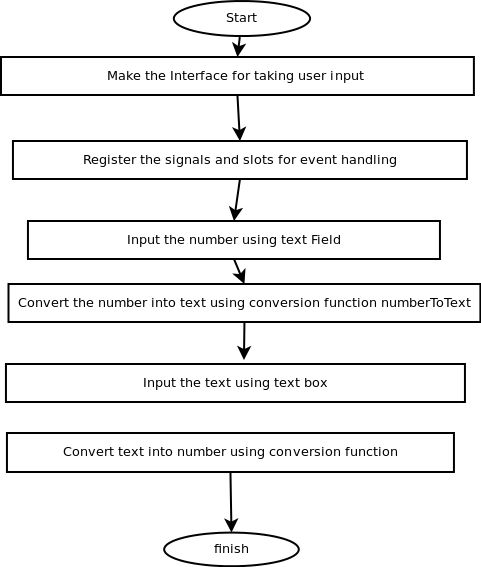
\includegraphics[height=14cm, width=12cm]{flowchart.png}

FIGURE 1: Flow Chart 
\end{center}-
\newpage
 
\section{Logic Implementation}
 The logic for Shell script is discussed below:
 
\begin{enumerate}
\item Initially the user has to pass folder path and extension type of the file to be searched. 
\item Open the user given folder and search for the subfolders with names having only small letters and without
spaces. cd and grep commands has been used for this.
\item In these subfolders, the names of files that have the user given extension are written into match.txt .
\item If the given extension is a c or sh, execute the files using gcc.
\item Convert all the capital letters to small case and remove blank spaces in the names of all the subfolders
of the given folder.
\item convert gif files into png in the subfolders which match pattern when the extension type is given gif.

  \end{enumerate}
 
 \newpage
 %Specifications and Assumptions
 \section{Execution Directives}
 
 The execution directives for executing the the scripts is given below:
  \begin{enumerate} 
 
 \item cd path of the  script 
 \item script name foldername extensiontype
 \item output will be saved in matter.txt in every subfolder.

 
  
  \end{enumerate}

 \newpage
 
 \section{Output}
 The snapshot of the output window after scriptname foldernamem extension type
  
\begin{center}
\vspace{1cm}
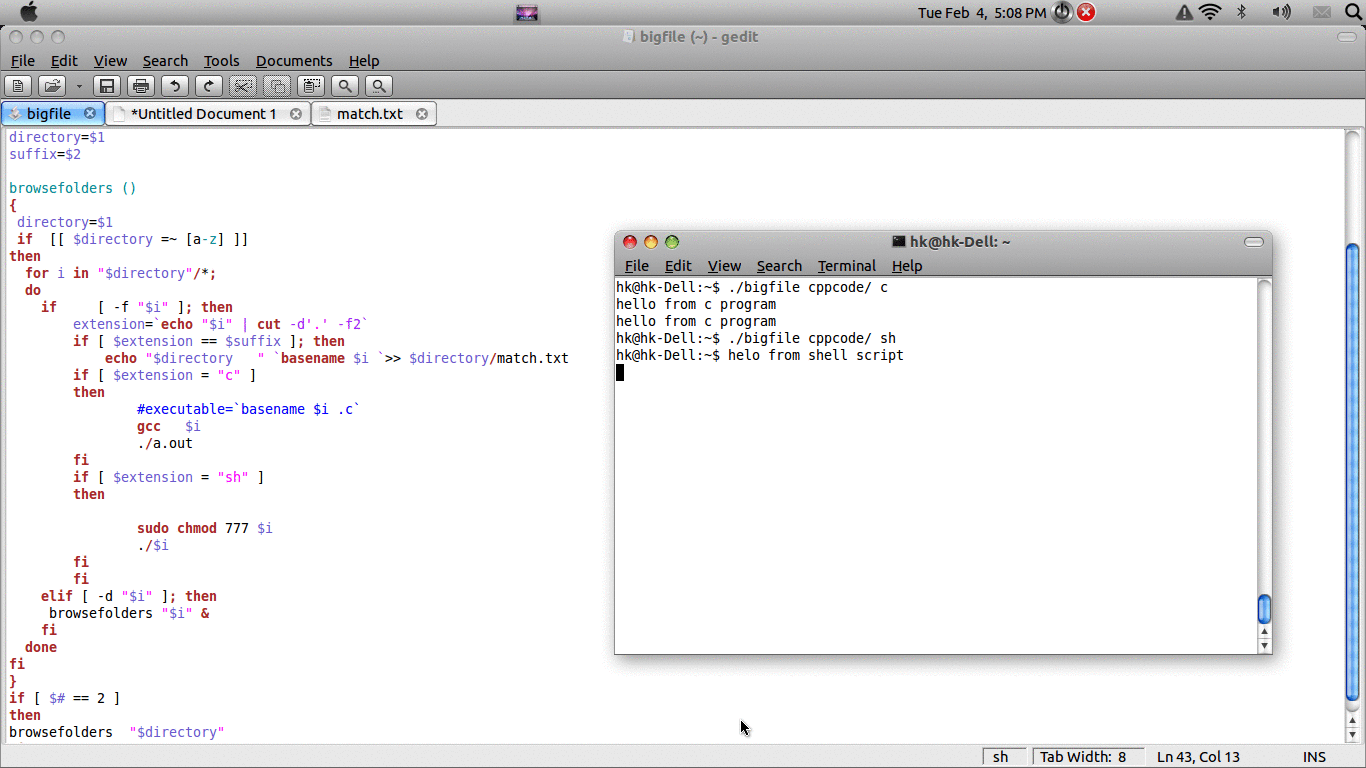
\includegraphics[height=12cm, width=12cm]{./Screenshot.png}

FIGURE 1: RESULT 
\end{center}-



 \newpage
  \section{Result And Conclusion}
The conclusions drawn from the above programs are given below:

\begin{enumerate}
 \item The problem seems to have been designed to provide hand on experience with the concepts of shell scripting. 
A shell script is a script written for the shell, or command line interpreter, of an operating system.
Scripts are collections of commands that are stored in a file. The shell can read this file and act on the commands as if they were typed at the keyboard.
 \item converted images into png are of good quality as they are converted using convert command .
\item if directory name has sapce it will be removed or capital letters will be converted into small letters in second case.
 
\end{enumerate}

 \end {document}